% latex article template

% cheat sheet(eng): http://www.pvv.ntnu.no/~walle/latex/dokumentasjon/latexsheet.pdf
% cheat sheet2(eng): http://www.pvv.ntnu.no/~walle/latex/dokumentasjon/LaTeX-cheat-sheet.pdf
% reference manual(eng): http://ctan.uib.no/info/latex2e-help-texinfo/latex2e.html

% The document class defines the type of document. Presentation, article, letter, etc. 
\documentclass[12pt, a4paper]{article}

% packages to be used. needed to use images and such things. 
\usepackage[pdfborder=0 0 0]{hyperref}
\usepackage[utf8]{inputenc}
\usepackage[english]{babel}
\usepackage{graphicx}
\PassOptionsToPackage{hyphens}{url}

% hides the section numbering. 
\setcounter{secnumdepth}{-1}

% Graphics/image lications and extensions. 
\DeclareGraphicsExtensions{.pdf, .png, .jpg, .jpeg}
\graphicspath{{./images/}}

% Title or header for the document. 
\title{
	Tiø4116, ex6
}
% Author
\author{
	Magnus L. Kirø \\
}
\date{\today}

\begin{document}
\maketitle
\pagenumbering{arabic}

\begin{abstract}
This is the paper's abstract \ldots
\end{abstract}

\section{Task 1}
\paragraph{a}
utgifter innland: 20 + 2 = 22 i gjeld etter år 1.
inntekt innland: -22 + 22 + 15.96 = 15.96 etter år 2.

utgifter utland: 10 + 1 + 1.1 = 12.1 i gjeld etter år 2.
inntekter innland = 28.05 - 12.1 = 15.95 etter år 2.

For innvesteringer hjemme vil utgiftene være dekket etter år 1. Da sitter man
igjen med en inntekt på 15.96 etter år 2.

For innvesteringen i utlandet vil man først etter år 2 ha dekket utgiftene. Da
sitter man igjen med 15.95 i inntekt. 

Man vil velge å innvestere hjemme. 

\paragraph{b}
Med endret rente til 15\% vil man innvestere hjemme.

\paragraph{c}
Når renten er på 5\% vil man innvestere i utlandet. Da får man høyere inntekt. 

\paragraph{d}
Nei, en renteøkning vil ikke alltid tilsi at man reduserer investeringen.
Man må se innvesteringen i sammenheng med perioden man er villig til å
innvestere. og ikke bare den korte to års perioden. 


\section{Task 2}
t1 = 245000, 
t6 = 265000,

t6 = -300000,
t7 = 320000 -t6,
t8..n = tn-1 *1.01 -t6,

Etter 40 år får vi en nåverdi for arbeid i byggebransjen lik: 4460568.35, mens
nåverdien av utdanning på ntnu er: 5645469.45

\section{Task 3}
\paragraph{a}
20 milliarder, 40år, +1.5 milliarder, 
900 MWh ==> 7884 GWh i året. 
driftskostnader = .05 kr per KWh
7\% diskontering.

Man må ha en pris på 39 øre per kWh for at anlegget skal gå godt økonomisk. 

\paragraph{b}
Med en strømpris på 65øre kan man maksimalt bruke 43064315509 kroner på
oppryddning.

\paragraph{c}
Ved å bygge et sikkert kraftverk vil man fortsatt gå godt i plus, og man vil ha
18064315509 i inntekter etter 40år. 

\section{Task 4}
\paragraph{a}
Ja, Nils kommer til å være interessert i kontantstrømmen.

\paragraph{b}
Årlig utvikling: 
saldo per år, fra år 0.
\begin{itemizt}
    \item 5
    \item 3.25
    \item 1.4125
    \item -0.516875
    \item -2.54271875
    \item -4.6698546875
    \item 0.0966525781
\end{itemize}

\paragraph{c}
Nils vil låne penger av Agnes i slutten av år 2. Han vil låne 4.67. 

\paragraph{d}
Nils vil ikke ta arven, da han må låne penger av Agnes. om han låner penger
kommer han dårligere ut enn om han ikke hadde tatt noe. Selv med en rente på
5.5\% fra Agnes vil det ikke lønne seg for Nils å ta arven. 

\section{Task 5}
\paragraph{a} se bildet
\begin{figure}[htb]
    \centering
    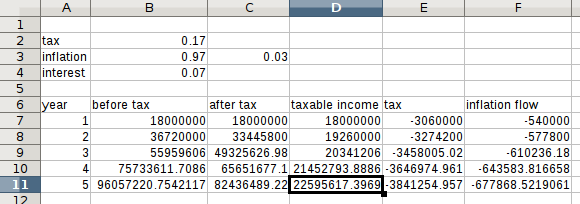
\includegraphics[width=\textwidth]{cashflow} 
    \label{fig:Cashflow}
\end{figure}

\paragraph{b}
Gitt at man vil beholde hele gevinsten på 18 millioner i året, så sitter man
igjen med 6 millioner i gevinst på renter o.l, noe man kan bruke på produskjons
enheten. 

\section{Task 6}
De årlig innskuddene blir på 688NOK. 
diskonteringen: =SUM(C2 /(1.045^A2))


se bilde
\begin{figure}[htb]
    \centering
    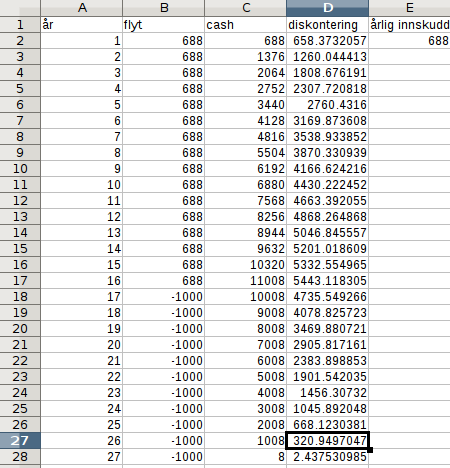
\includegraphics[width=\textwidth]{part6}
    \label{fig:part6}
\end{figure}


\end{document}
This is never printed
